\documentclass{article}

% -------------------
% Packages
% -------------------
\usepackage[a4paper,left=15mm,right=15mm,top=25mm,bottom=25mm]{geometry}
\usepackage[UTF8]{ctex}
\usepackage{graphicx}
\usepackage{amsmath}
\usepackage{float}
\usepackage{color}
\usepackage{listings}
%\usepackage{textcomp}
%\usepackage[framed,numbered,autolinebreaks,useliterate]{mcode}    
\usepackage{xcolor}
\usepackage[colorlinks=true,linkcolor=black, citecolor=blue, urlcolor=blue]{hyperref}
%\setcounter{secnumdepth}{3}
\setcounter{tocdepth}{2}

% -------------------
% Title Informations
% -------------------
\title{uEMEP模型使用参考手册}

\author{常鸣$^1$, 穆青$^2$, 郑炼明$^1$, 马明睿$^1$, 张兴腾$^1$, 王雪梅$^1$, Bruce Rolstad Denby$^2$, Michael Gauss$^2$}
\date{%
      $^1$暨南大学环境与气候研究院\\%
      $^2$挪威气象局\\[2ex]%
      \today
     }

% -------------------
% Content
% -------------------
\begin{document}

\maketitle

%\section{致谢}

uEMEP模型是针对城市尺度空气污染研发的、将欧洲长期使用的EMEP MSC-W中尺度空气质量模型的结果基于经典高斯模型进行降尺度计算的一个新工具。我们尝试撰写这份中文使用参考手册以帮助uEMEP模型学习者更快的掌握这一工具,期望引入更多的气象、环保工作者参与到uEMEP模型的研发中,从而更好的支撑城市空气质量预报工作。这份手册的编制得到了中挪合作项目AirQuip的资助。

\tableofcontents
\newpage

\section{模型计算过程}

{\color{red} 需要穆青考虑下这部分内容的设计}

uEMEP计算过程的理论基础译自《Development and implementation of uEMEP》(Bruce Rolstad Denby, Peter Wind, Michael Gauss, Hilde Fargeli, Alvaro Valdebenito, Agnes Nyiri, Heiko Klein, Qing Mu, Eivind Grøtting Wærsted著)。

\subsection{总体概念和方法}

\subsection{降尺度方法}

\begin{figure}[H]
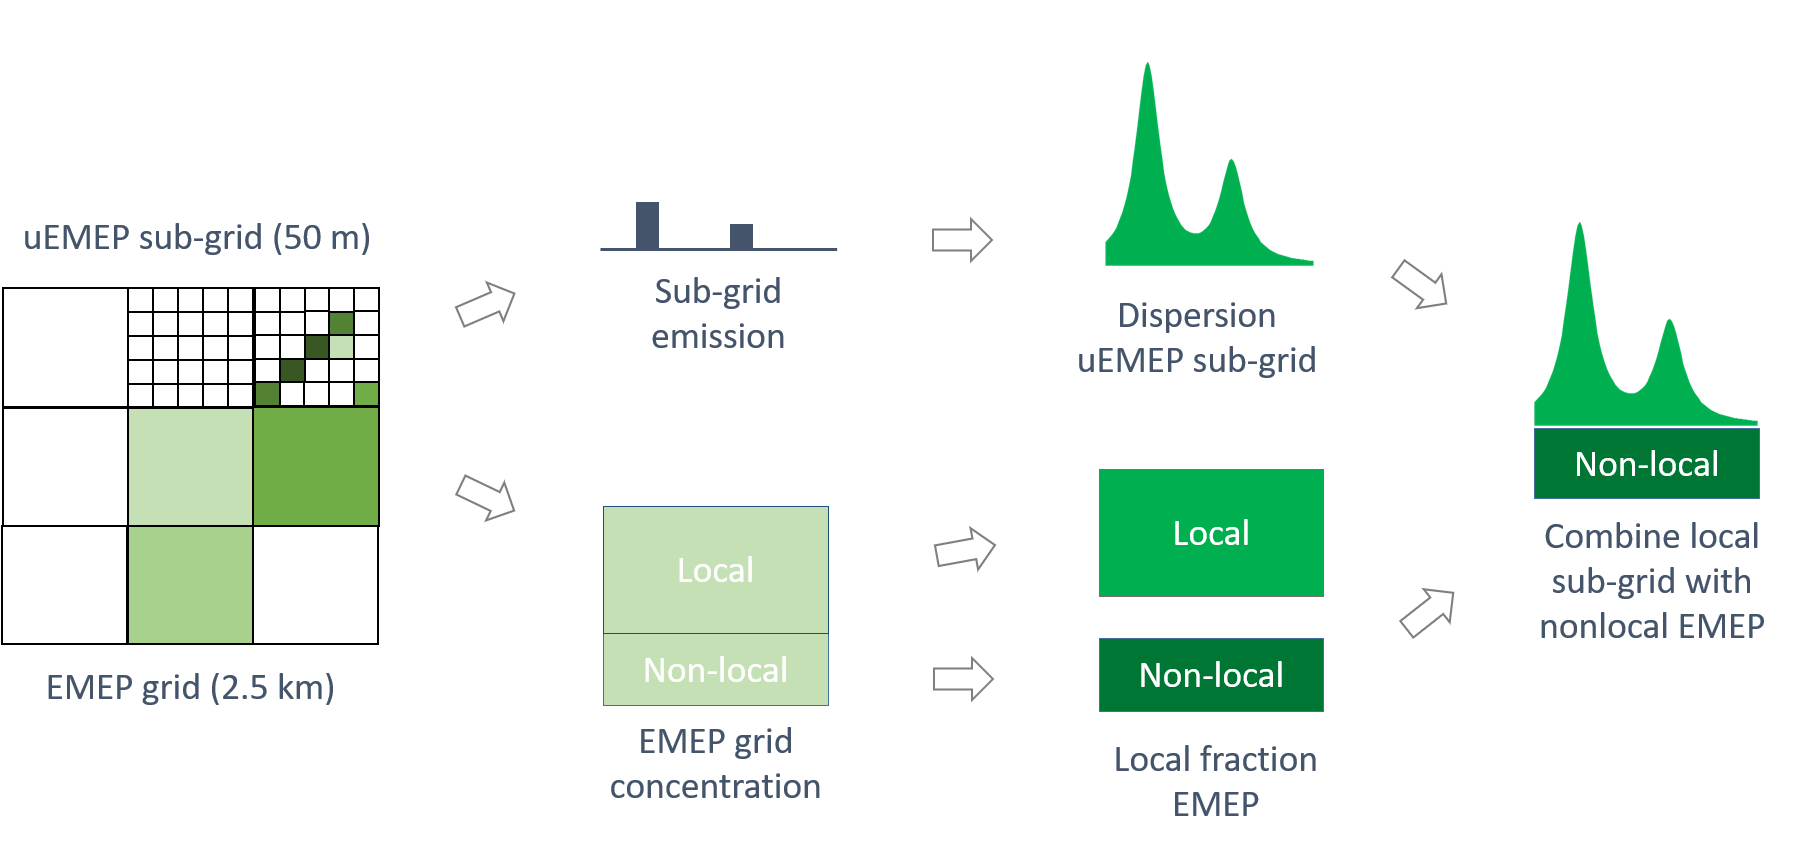
\includegraphics[width=0.9\textwidth]{fig11.png}
\centering\caption{降尺度方法概念图}\label{fig11}
\end{figure}

\subsubsection{污染物浓度重分配}
\subsubsection{本地排放源的置换}

\subsection{排放贡献计算}

\subsubsection{中尺度模式本地贡献比例的计算}
\subsubsection{本地和外来贡献的滑动窗口设置}

\begin{figure}[H]
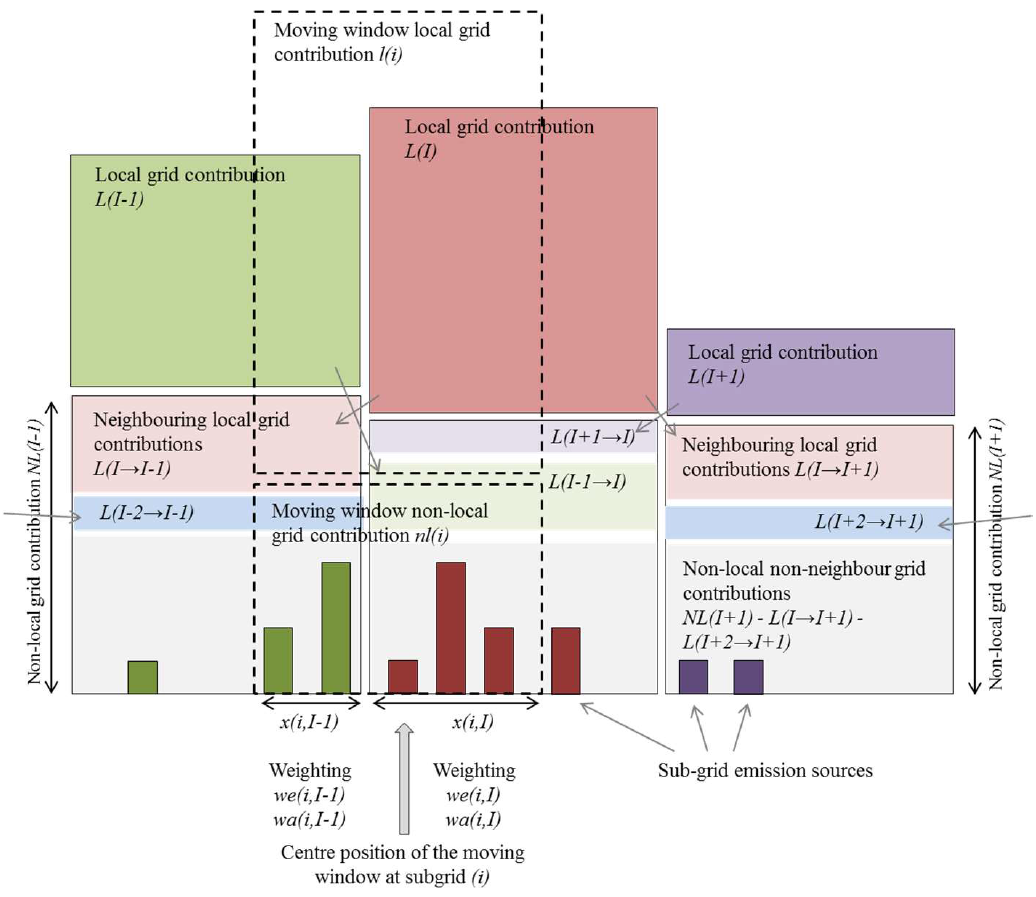
\includegraphics[width=0.9\textwidth]{fig1.png}
\centering\caption{滑动窗口剖面示意图}\label{fig1}
\end{figure}

\subsection{次网格高斯扩散模型}

\subsection{其他参数化过程}

\section{模型运行设置}

{\color{red} 常鸣、张兴腾撰写}

\begin{figure}[H]
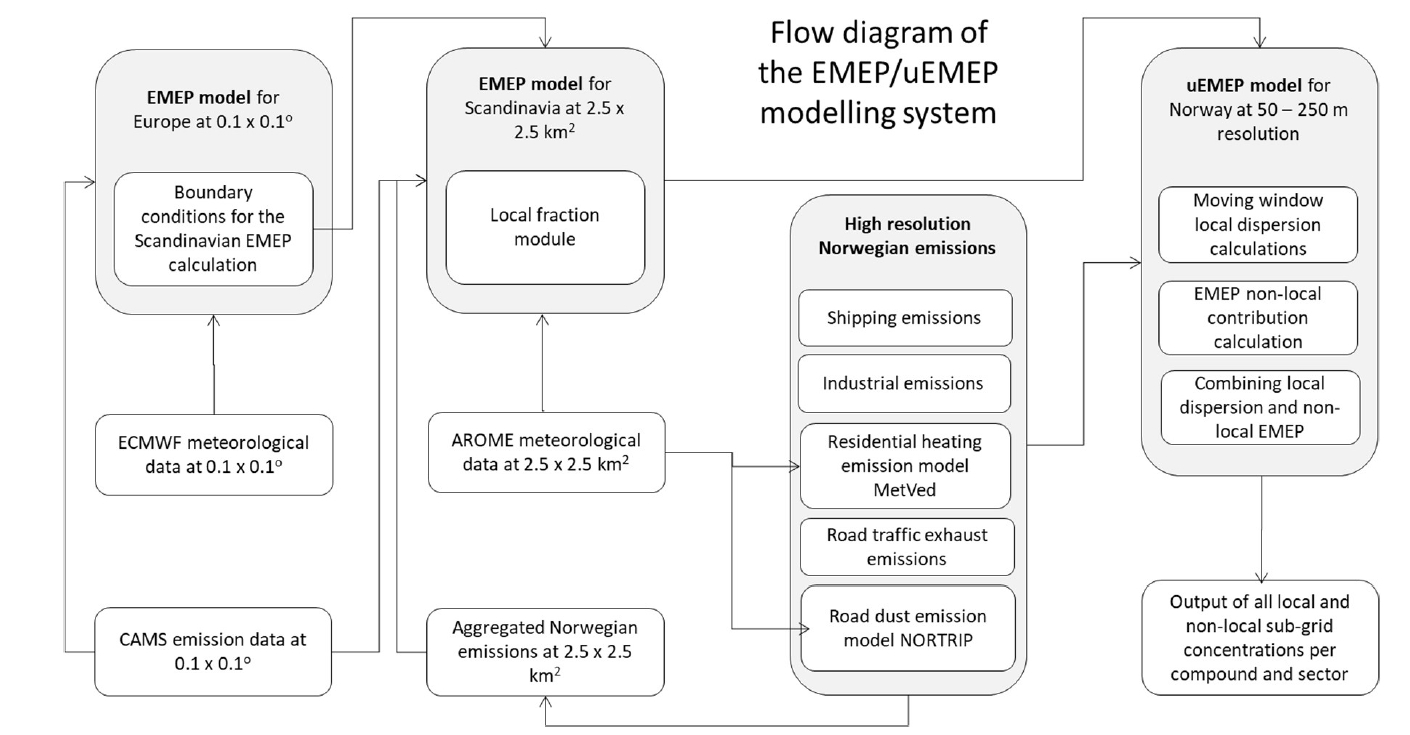
\includegraphics[width=0.9\textwidth]{emepuemepflow.png}
\centering\caption{模式运行过程示意}\label{emepuemepflow}
\end{figure}

\subsection{模型安装步骤}

\begin{itemize}

\item 代码下载

uEMEP目前为开放获取的开源模型,其源代码存放在了GitHub上。因此,使用者需要首先对命令行操作及Git等命令有一定的基础\footnote{\href{https://www.liaoxuefeng.com/wiki/896043488029600}{Git简明教程}}。

uEMEP模型具体下载路径为:\url{https://github.com/metno/uEMEP}。

使用如下命令将uEMEP源代码Clone到本地:

\begin{lstlisting}[language={[ANSI]C},keywordstyle=\color{blue!70},commentstyle=\color{red!50!green!50!blue!50},frame=shadowbox, rulesepcolor=\color{red!20!green!20!blue!20}]
git clone https://github.com/metno/uEMEP.git
\end{lstlisting}

\item 环境设置

\item 编译安装

\end{itemize}

\subsection{模型运行步骤}

\begin{itemize}

\item 时间设置

\item 路径设置

\item 运行设置

\item 批量作业

\item 记录查看

\end{itemize}

\subsection{控制文件说明}

\subsection{源码内容说明}

\subsubsection{函数调用关系}

\subsubsection{函数用途}

\begin{itemize}

\item Makefile:
声明编译所用的fortran编译器,调用了Makefile.SRCS和dependencies用于声明编译关系。默认编译器为ifort,在JNU的HPC上测试通过。

\item Area\_weighted\_interpolation\_function.f90:
空间权重插值函数。

\item lambert\_projection.f90:
兰伯特投影转换函数。

\item rdm2ll.f90:
Rijksdriehoek投影(EPSG 28992)转为WGS1984坐标系的转换函数。一般我国国内用不到。

\item read\_esri\_ascii\_file.f90:
读取Esri的ArcGIS或ENVI导出文本文件的函数。包含五个subroutine,分别为读头文件、读/写二维ascii、读/写三维ascii。

\item uEMEP\_Kz\_function.f90:
计算Kz和风廓线的函数。包含如下几个subroutine:uEMEP\_set\_dispersion\_sigma\_Kz,Kz\_func,z\_centremass\_gauss\_func,u\_profile\_val\_func,u\_profile\_neutral\_val\_func,phi\_func,phim\_func,phih\_func,z\_centremass\_gauss\_array\_func。

\item uEMEP\_aggregate\_proxy\_emission\_in\_EMEP\_grid.f90:
用于统计次网格排放量并且将它们与EMEP网格中的排放量进行交叉检验。

\end{itemize}

\section{输入数据说明}

{\color{red} 常鸣、郑炼明撰写}

\subsection{EMEP模式输出数据}

\subsection{本地排放清单资料}

\subsubsection{需要准备的排放数据类型}

\begin{itemize}

\item 道路移动源

\item 燃烧源

\item 工业过程源

\item 船舶源

\item 居民源

\end{itemize}

\subsubsection{排放数据格式转换}

\section{模拟性能评估}

\subsection{评估方法}

\subsection{研究案例}

\section{常见问题}

\section{参考文献}

%This work has been supported by the AirQuip project funded by the Research Council of Norway (Project Number: 267734).

\end{document}



